\documentclass{standalone}
\usepackage{tikz}
\usetikzlibrary{positioning}

\begin{document}

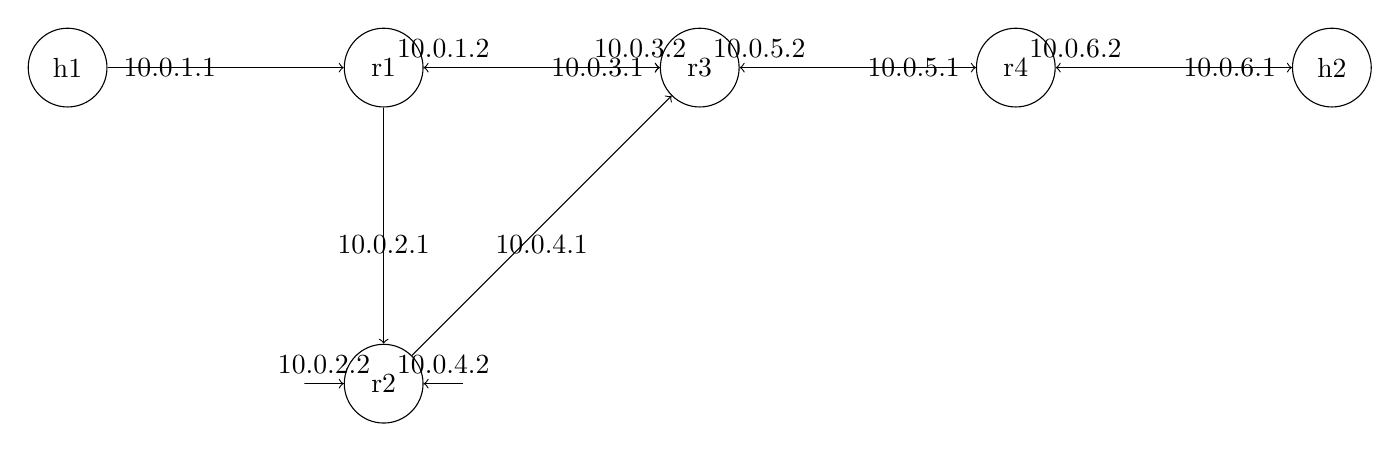
\begin{tikzpicture}[node distance=3cm]

    % 定义节点
    \node[circle, draw, minimum size=1cm] (h1) {h1};
    \node[circle, draw, minimum size=1cm] (r1) [right=of h1] {r1};
    \node[circle, draw, minimum size=1cm] (r2) [below=of r1] {r2};
    \node[circle, draw, minimum size=1cm] (r3) [right=of r1] {r3};
    \node[circle, draw, minimum size=1cm] (r4) [right=of r3] {r4};
    \node[circle, draw, minimum size=1cm] (h2) [right=of r4] {h2};

    % 连接节点并标注 IP
    \draw[->] (h1) -- (r1) node[midway, left] {10.0.1.1};
    \draw[->] (r1) -- (r2) node[midway, below] {10.0.2.1};
    \draw[->] (r1) -- (r3) node[midway, right] {10.0.3.1};
    \draw[->] (r2) -- (r3) node[midway, below] {10.0.4.1};
    \draw[->] (r3) -- (r4) node[midway, right] {10.0.5.1};
    \draw[->] (r4) -- (h2) node[midway, right] {10.0.6.1};

    % 其他连接
    \draw[->] (r1.east) -- ++(0.5,0) node[midway, above] {10.0.1.2} -- (r1.east);
    \draw[->] (r2.west) -- ++(-0.5,0) node[midway, above] {10.0.2.2} -- (r2.west);
    \draw[->] (r3.west) -- ++(-0.5,0) node[midway, above] {10.0.3.2} -- (r3.west);
    \draw[->] (r2.east) -- ++(0.5,0) node[midway, above] {10.0.4.2} -- (r2.east);
    \draw[->] (r3.east) -- ++(0.5,0) node[midway, above] {10.0.5.2} -- (r3.east);
    \draw[->] (r4.east) -- ++(0.5,0) node[midway, above] {10.0.6.2} -- (r4.east);

\end{tikzpicture}

\end{document}
